\section{Equipment and Method}
\label{sec:equip}

Table~\ref{tab:equip} lists the equipment. BESOS was assembled following the CAOS drawings~\cite{besos,guide} (Fig.~\ref{fig:setup}), with the \SI{30}{\milli\meter} doublet as collimator and the \SI{40}{\milli\meter} doublet as camera objective. A \SI{50}{\milli\meter} lens placed about \SI{50}{\milli\meter} in front of the slit concentrated the light of each source on it. The camera was focused with the red LED placed far from the instrument, minimizing the width of its slit image.

\begin{table}[htbp]
\caption{Equipment used in the experiment.}
\label{tab:equip}
\centering
\footnotesize
\begin{tabular}{@{}p{0.52\linewidth}p{0.42\linewidth}@{}}
\toprule
\textbf{Item} & \textbf{Use} \\
\midrule
BESOS head: slit \SI{25}{\micro\meter}$\times$\SI{3}{\milli\meter}; collimator doublet $f=\SI{30}{\milli\meter}$; SF18 prism, $A=60^\circ$, \SI{15}{\milli\meter}; camera doublet $f=\SI{40}{\milli\meter}$ & instrument under test \\
Lens $f=\SI{50}{\milli\meter}$ & feeds the slit \\
DMK 41AU02.AS (Sony ICX205AL CCD, $1280\times960$, \SI{4.65}{\micro\meter}, 8 bit) & spectrum camera \\
DMK 21AU04.AS ($640\times480$, \SI{5.6}{\micro\meter}) & slit viewer (alignment) \\
Blue, green and red LEDs & alignment, calibration check \\
Ar and Kr spectral lamps & wavelength calibration, resolution \\
Phone LED flash & continuum source (range) \\
AstroDMx Capture 2.17.2 & FITS acquisition \\
Python (numpy, scipy, astropy) & data reduction \\
\bottomrule
\end{tabular}
\end{table}

\begin{figure}[htbp]
\centering
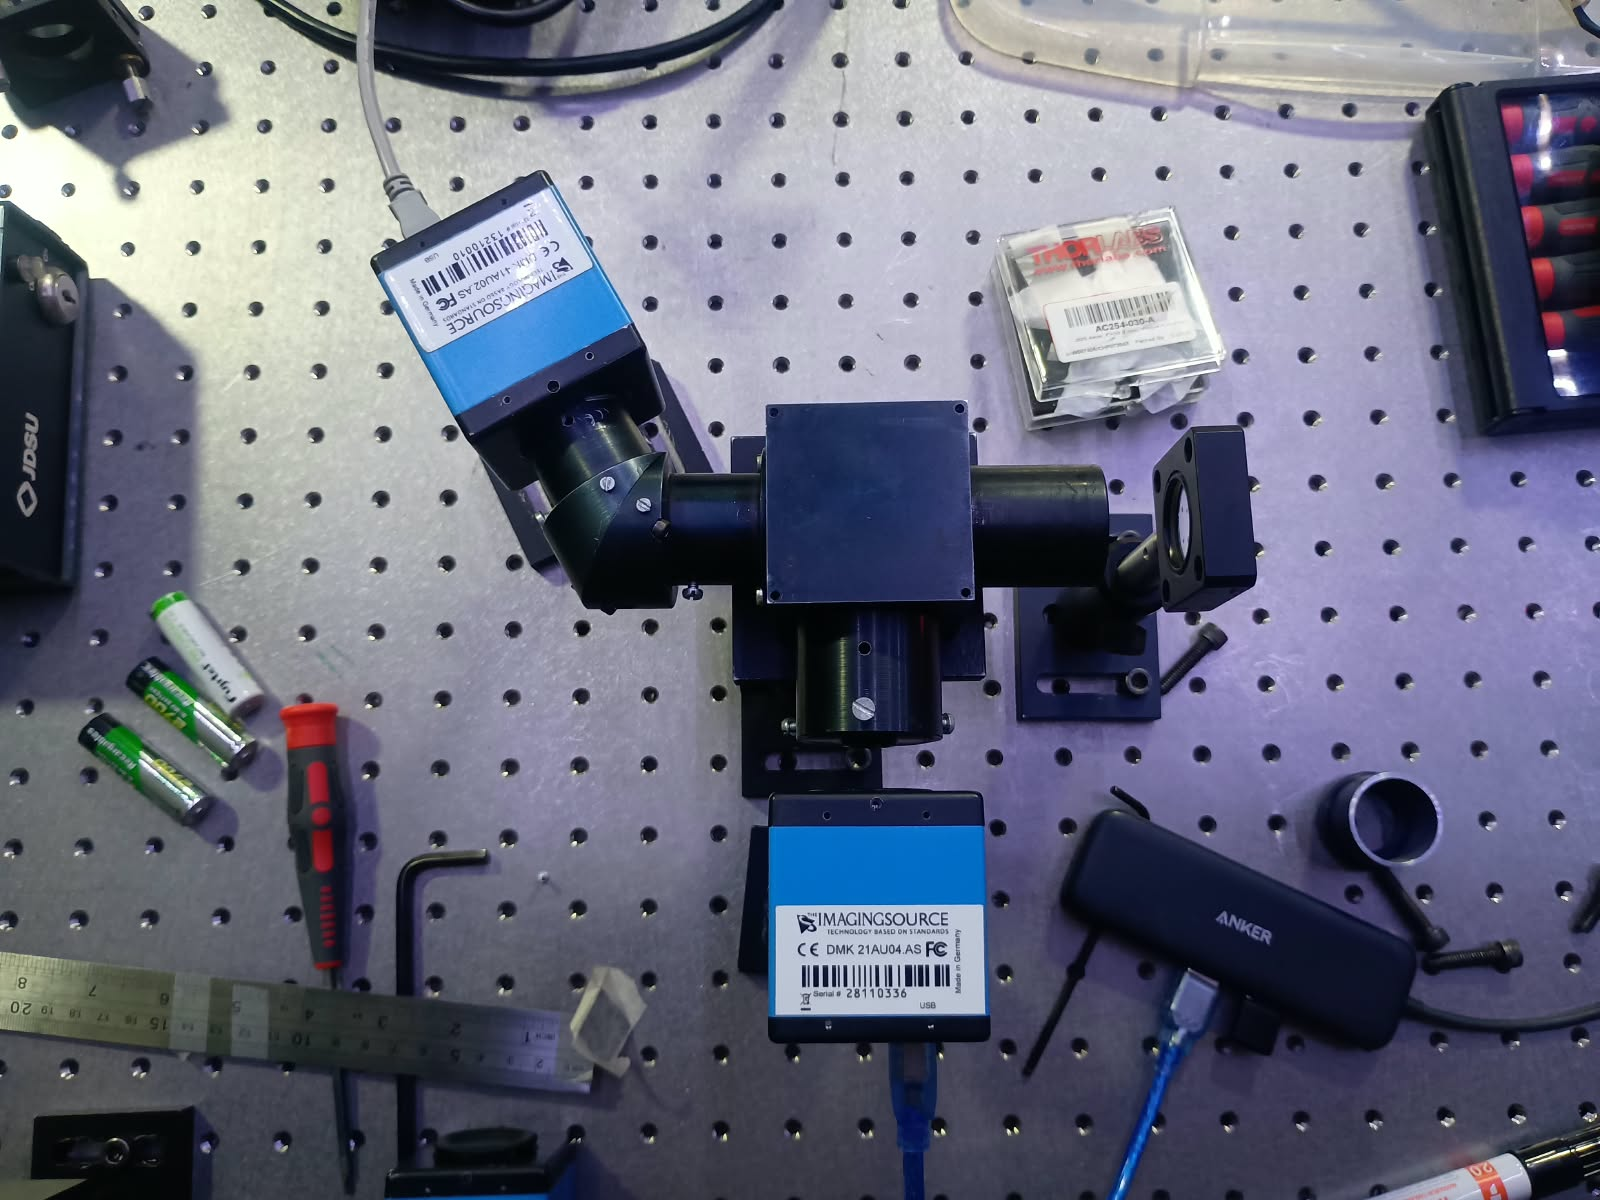
\includegraphics[width=0.85\linewidth]{montaje_besos.jpeg}
\caption{Setup: BESOS head (centre), spectrum camera DMK~41AU02.AS on the inclined port (top left), slit-viewer camera DMK~21AU04.AS (bottom) and the feeding lens mount (right).}
\label{fig:setup}
\end{figure}

For each source \NFrames{} frames were taken (gain 354--392, gamma 104, \SIrange{1}{150}{\milli\second} exposure, chosen to avoid saturation except for the flash). The reduction, implemented in a Python package, proceeds as follows: (i) median combination of the frames; (ii) tracing of a Kr line row by row and quadratic fit $x(y)$, used to shift every row so that the curved lines become vertical; (iii) extraction of the 1D spectrum averaging rows 450--550, the best-focus region; (iv) Gaussian fits, simultaneous for blended features; (v) Hartmann calibration~\eqref{eq:hartmann} with isolated Ar and Kr lines; (vi) computation of $P$, $R$ and the range, and comparison with \eqref{eq:prism}--\eqref{eq:range}.
